%%%%%%%%%%%%%%%%%%%%%%%%%%%%%%%%%%%%%%%%%%%%%%%%%%%%%%%%%%%%%%%%%%%%%
%%                                                                 %%
%% Please do not use \input{...} to include other tex files.       %%
%% Submit your LaTeX manuscript as one .tex document.              %%
%%                                                                 %%
%% All additional figures and files should be attached             %%
%% separately and not embedded in the \TeX\ document itself.       %%
%%                                                                 %%
%%%%%%%%%%%%%%%%%%%%%%%%%%%%%%%%%%%%%%%%%%%%%%%%%%%%%%%%%%%%%%%%%%%%%

\documentclass[sn-basic]{sn-jnl}% referee option is meant for double line spacing

%%=======================================================%%
%% to print line numbers in the margin use lineno option %%
%%=======================================================%%

%%\documentclass[lineno,sn-basic]{sn-jnl}% Basic Springer Nature Reference Style/Chemistry Reference Style

%%======================================================%%
%% to compile with pdflatex/xelatex use pdflatex option %%
%%======================================================%%

%%\documentclass[pdflatex,sn-basic]{sn-jnl}% Basic Springer Nature Reference Style/Chemistry Reference Style

%%\documentclass[sn-basic]{sn-jnl}% Basic Springer Nature Reference Style/Chemistry Reference Style
%%\documentclass[sn-mathphys]{sn-jnl}% Math and Physical Sciences Reference Style
%%\documentclass[sn-aps]{sn-jnl}% American Physical Society (APS) Reference Style
%%\documentclass[sn-vancouver]{sn-jnl}% Vancouver Reference Style
%%\documentclass[sn-apa]{sn-jnl}% APA Reference Style
%%\documentclass[sn-chicago]{sn-jnl}% Chicago-based Humanities Reference Style
%%\documentclass[sn-standardnature]{sn-jnl}% Standard Nature Portfolio Reference Style
%%\documentclass[default]{sn-jnl}% Default
%%\documentclass[default,iicol]{sn-jnl}% Default with double column layout



%%%% Standard Packages
%%<additional latex packages if required can be included here>
%%%%

%%%%%=============================================================================%%%%
%%%%  Remarks: This template is provided to aid authors with the preparation
%%%%  of original research articles intended for submission to journals published 
%%%%  by Springer Nature. The guidance has been prepared in partnership with 
%%%%  production teams to conform to Springer Nature technical requirements. 
%%%%  Editorial and presentation requirements differ among journal portfolios and 
%%%%  research disciplines. You may find sections in this template are irrelevant 
%%%%  to your work and are empowered to omit any such section if allowed by the 
%%%%  journal you intend to submit to. The submission guidelines and policies 
%%%%  of the journal take precedence. A detailed User Manual is available in the 
%%%%  template package for technical guidance.
%%%%%=============================================================================%%%%

\jyear{2023}%
%\usepackage{subcaption}  
\usepackage{subfigure}
\usepackage{rotating}
%% as per the requirement new theorem styles can be included as shown below
\theoremstyle{thmstyleone}%
\newtheorem{theorem}{Theorem}%  meant for continuous numbers
%%\newtheorem{theorem}{Theorem}[section]% meant for sectionwise numbers
%% optional argument [theorem] produces theorem numbering sequence instead of independent numbers for Proposition
\newtheorem{proposition}[theorem]{Proposition}% 
%%\newtheorem{proposition}{Proposition}% to get separate numbers for theorem and proposition etc.

\theoremstyle{thmstyletwo}%
\newtheorem{example}{Example}%
\newtheorem{remark}{Remark}%

\theoremstyle{thmstylethree}%
\newtheorem{definition}{Definition}%

\raggedbottom
%%\unnumbered% uncomment this for unnumbered level heads

\begin{document}

\title[Waning of Immunity against COVID-19]{Waning of Vaccination, Post-Infection and Hybrid Immunity against Severe Outcomes of Omicron: A Population Study TBDJT(asi pls změň)}

%%=============================================================%%
%% Prefix	-> \pfx{Dr}
%% GivenName	-> \fnm{Joergen W.}
%% Particle	-> \spfx{van der} -> surname prefix
%% FamilyName	-> \sur{Ploeg}
%% Suffix	-> \sfx{IV}
%% NatureName	-> \tanm{Poet Laureate} -> Title after name
%% Degrees	-> \dgr{MSc, PhD}
%% \author*[1,2]{\pfx{Dr} \fnm{Joergen W.} \spfx{van der} \sur{Ploeg} \sfx{IV} \tanm{Poet Laureate} 
%%                 \dgr{MSc, PhD}}\email{iauthor@gmail.com}
%%=============================================================%%

\author*[1,2]{\fnm{Jan} \sur{Trnka}}\email{jan.trnka@lf3.cuni.cz} \equalcont{These authors contributed equally to this work.}
\author[3]{\fnm{Tamara} \sur{Barusová}}\email{barusova@biostatistika.cz,} \equalcont{These authors contributed equally to this work.}
\author[4,5]{\fnm{Jiří} \sur{Jarkovský}}\email{jiri.jarkovsky@uzis.cz} \equalcont{These authors contributed equally to this work.}
\author[4,5]{\fnm{Ondřej} \sur{Májek}}\email{ondrej.majek@uzis.cz} \equalcont{These authors contributed equally to this work.}
\author[4,5]{\fnm{Tomáš} \sur{Pavlík}}\email{pavlik@iba.muni.cz} \equalcont{These authors contributed equally to this work.}
\author[6]{\fnm{Lenka} \sur{Přibylová}}\email{pribylova@math.muni.cz} \equalcont{These authors contributed equally to this work.}
\author[7]{\fnm{Josefína} \sur{Weinerová}}\email{josefina.weinerova@nottingham.ac.uk} \equalcont{These authors contributed equally to this work.}
\author[2,8]{\fnm{Milan} \sur{Zajíček}}\email{zajicek@utia.cas.cz} \equalcont{These authors contributed equally to this work.}
\author[2,8]{\fnm{Martin} \sur{Šmíd}}\email{smid@utia.cas.cz} \equalcont{These authors contributed equally to this work.}

\affil[1]{\orgdiv{Department of Biochemistry, Cell and Molecular Biology}, \orgname{Third Faculty of Medicine, Charles University}, \orgaddress{\street{TBDStreet}, \city{Prague}, \postcode{TBDPSC}, \country{Czech Republic}}}
\affil[2]{\orgname{Centre for Modelling of Biological and Social Processes}, \orgaddress{\street{Na Břehu 15}, \city{Prague 9}, \postcode{190 00}, \country{Czech Republic}}}
\affil[3]{\orgname{Institute of Biostatistics and Analyses}, \orgaddress{\street{Poštovská 68/3}, \city{Brno}, \postcode{602 00}, \country{Czech Republic}}}
\affil[4]{\orgdiv{Institute of Biostatistics and Analyses}, \orgname{Faculty of Medicine, Masaryk University}, \orgaddress{\street{TBDStreet}, \city{Brno}, \postcode{TBDPSC}, \country{Czech Republic}}}
\affil[5]{\orgdiv{Department of Data Analysis}, \orgname{Institute of Health Information and Statistics of the Czech Republic}, \orgaddress{\street{TBDStreet}, \city{Pragueš}, \postcode{TBDPSC}, \country{Czech Republic}}}
\affil[6]{\orgdiv{Department of Mathematics and Statistics}, \orgname{Faculty of Science, Masaryk University}, \orgaddress{\street{TBDStreet}, \city{Brno}, \postcode{TBDPSC}, \country{Czech Republic}}}
\affil[7]{\orgdiv{School of Psychology}, \orgname{University of Nottingham}, \orgaddress{\street{TBDStreet}, \city{Nottingham}, \postcode{NG7 2RD}, \country{United Kingdom}}}
\affil[8]{\orgdiv{Department of Econometrics}, \orgname{Institute of Information Theory and Automation, Czech Academy of Sciences}, \orgaddress{\street{Pod Vodárenskou věží 4}, \city{Prague 8}, \postcode{182 00}, \country{Czech Republic}}}

%%==================================%%
%% sample for unstructured abstract %%
%%==================================%%

\abstract{This study evaluates the effectiveness of different types of immunity against Omicron infections and long covid in the Czech Republic based on population data. The findings suggest that hybrid and post-infection immunity provide a slowly waning protection against both severe course and long covid, with stronger protection against the former. Booster vaccinations offer a strong but quickly waning protection against the virus, while sole vaccination is weak and insignificant for BA45 and newer variants. }

%%================================%%
%% Sample for structured abstract %%
%%================================%%

% \abstract{\textbf{Purpose:} The abstract serves both as a general introduction to the topic and as a brief, non-technical summary of the main results and their implications. The abstract must not include subheadings (unless expressly permitted in the journal's Instructions to Authors), equations or citations. As a guide the abstract should not exceed 200 words. Most journals do not set a hard limit however authors are advised to check the author instructions for the journal they are submitting to.
% 
% \textbf{Methods:} The abstract serves both as a general introduction to the topic and as a brief, non-technical summary of the main results and their implications. The abstract must not include subheadings (unless expressly permitted in the journal's Instructions to Authors), equations or citations. As a guide the abstract should not exceed 200 words. Most journals do not set a hard limit however authors are advised to check the author instructions for the journal they are submitting to.
% 
% \textbf{Results:} The abstract serves both as a general introduction to the topic and as a brief, non-technical summary of the main results and their implications. The abstract must not include subheadings (unless expressly permitted in the journal's Instructions to Authors), equations or citations. As a guide the abstract should not exceed 200 words. Most journals do not set a hard limit however authors are advised to check the author instructions for the journal they are submitting to.
% 
% \textbf{Conclusion:} The abstract serves both as a general introduction to the topic and as a brief, non-technical summary of the main results and their implications. The abstract must not include subheadings (unless expressly permitted in the journal's Instructions to Authors), equations or citations. As a guide the abstract should not exceed 200 words. Most journals do not set a hard limit however authors are advised to check the author instructions for the journal they are submitting to.}


\keywords{keyword1, Keyword2, Keyword3, Keyword4}

%%\pacs[JEL Classification]{D8, H51}

%%\pacs[MSC Classification]{35A01, 65L10, 65L12, 65L20, 65L70}

\maketitle

\section{Introduction}\label{sec1}

With COVID-19 becoming endemic, quantification of protection by various sources of immunity is necessary, be it post-infection--, post-vaccination-- or hybrid immunity. In this study, we focus on two undesirable outcomes of the disease: severe course needing oxygen support and Long Covid. 

Previous work on immunity against severe course includes whole-population observation study \citep{smid2022protection}, meta-studies \citep{wu2022long,yang2023efficacy}, the former surveying both controlled trials and observational studies, the latter only controlled trials. These works study the effectiveness/efficacy of primary series and booster doses against infection, hospitalization, severe course, and death due to COVID-19. In the present paper, we, in addition, study the waning of post-infection and hybrid immunity; yet these have been studied by  \citep{smid2022protection}, results therein are inaccurate, moreover comparing the protection only during two time-intervals. As of our knowledge, our study is the first to describe waning patterns up to 18 months (compared to at most 10 months in the existing studies), deals with second boosters, and works with recent data, starting from BA45 variant emergence in summer 2022. 

The research into the impact of vaccination on Long Covid symptom development has so far produced mixed results. A retrospective study conducted on Israeli healthcare services data found that vaccinated individuals who contracted SARS-CoV-2 were not at significantly lower risk of Long Covid symptoms save for prolonged dyspnoea (i.e. shortness of breath)compared to unvaccinated people with SARS-CoV-2 \citep{mizrahi2023long}. A recent meta-analysis \citep{tsampasian2023risk} examined a range of risk factors associated with Long Covid symptoms. The sample included 4 studies containing in total 249,788 patients which examined the effect of vaccination status. The meta-analysis found that those who have been vaccinated with two doses prior to infection had a 40\% lower risk of developing Long Covid symptoms compared to unvaccinated infected individuals \citep{tsampasian2023risk}. In addition, \cite{al2022long} also found that the risk of Long Covid symptoms was lower for individuals vaccinated than those who were unvaccinated prior to infection for 24 out of 47 symptoms studied \citep{al2022long}. These findings suggest that vaccination does provide some level of protection against Long Covid development which may potentially affect only certain symptoms of Long Covid. It is of note that all of the previous studies focus only on the infected population and compare vaccinated and unvaccinated subgroups. We focus on both this comparison and also on overall population of infected and not infected. This allows us to study the effect of vaccination on Long Covid not only in terms of whether it influences the development of Long Covid in infected individuals but also how it protects against Long Covid through avoiding the SARS-CoV-2 infection in the first place.


\section{Data}

Data for the study comes from the Czech National Information System of Infectious Diseases (ISID), containing records of all positive SARS-CoV-2 cases in the Czech Republic, including children. The ISID database collects demographic data (age, sex, and region of residence), vaccination history, infection, and reinfection dates, hospitalization information including treatment type TBDUZIS and an indicator, issued by hospital personnel, of whether or not the primary reason for hospitalization was COVID, and death date. For a part of infections, the data includes information on variants based on a variant identification using the definition of viral S-protein mutations
according to the European Centre for Disease Prevention
and Control \cite{ECDC_var_concern}. The data also include information on whether and when the individual was diagnosed with long covid. TBDUZIS(prosím popište)
Selected records, which however include all the infected individuals, include a commorbidity index TBDUZIS(prosím upřesněte). Data of death from whatever reason is only used for censoring purposes and is obtained from the Death Certificate System. To have whole population data, individuals not recorded in the database have been added to the dataset using public data from the Czech Statistical Office. 

TBDUTIA(popisna statistika)

\section{Methods}

We analyzed two undesirable outcomes related to SARS-CoV-2 infection: (1) severe course, indicated by the fact of using any oxygen therapy within 30 days from the positive test together and confirmation that the primary reason for hospitalization was COVID-19, (2) the long covid diagnosis following infection by no more than 183 days (half year).

We are only studying outcomes related to Omicron variants, and we are identifying infections as either BA1/2, or BA4/5+ (BA4/5 and later variants). As BA1/2 infections, we consider those that were identified as such by allele-specific PCR method or those that tested positive during the period from January 31, 2022, to May 23, 2022, when the BA1/2 variant was predominant in the Czech Republic, with a prevalence above 94\% according to sequencing method\footnote{Global Initiative on Sharing Avian Influenza Data (GISAID). (2023). SARS-CoV-2 sequence data. Retrieved from https://www.gisaid.org/ via covariants.org. \label{fnlabel}}. As BA4/5+ infections, we consider those that were identified as BA4/5 infections by allele-specific PCR method or those that were identified from August 1, 2022, to October 24, 2022, during the period when the BA4/5 variant was predominant in the Czech Republic, with a prevalence above 95\%\footref{fnlabel}; + express that we also include infections that occurred later, when the Omicron variants, including XBB and BQ.1, were still dominating along with BA4/5, accounting for almost 100\% of COVID-19 cases\footref{fnlabel}.
Due to our half-year [lhůtě na rozhodnutí, jestli je to LC] we take only infections by BA1/2 into account when studying the long covid.

To compute the effectiveness/protection against the severe course,  we used Cox regression analysis with time-varying covariates and calendar time applied to the whole population, analogously to \cite{smid2022protection}. We took infections as recurring events. For each source of immunity, we split the follow-up into as much as nine 61-day time windows, i.e. we estimated up to 18-month waning patterns; however, for some immunity sources, such as boosters, the patterns are shorter due to their late introduction. Control variables were age group and sex.

We perform two types of analyses of long-covid: the one applied to the whole population, in which we use Cox regression analogously as above. The outcome here is an infection followed by the long-covid diagnosis. In the second type of analysis, we study the outcome (long covid diagnosis by 183 days) within all the individuals infected by BA1/2. Here, we evaluate the protection/effectiveness by a logistic regression with the same covariates plus the comorbidity index as an additional control variable. The former analysis deals with risk of suffereing long-covid of still unifected individual, while the latter examines the risk of suffering long-covid once being infected.


\section{Results}

If Figure \ref{trends}, protection levels and waning patterns of various immunity types are depicted, and, in Figure \ref{heatmaps}, overall differences in protection levels are displayed. 

\subsection{Severe Course}

For severe course, generally, all immunity types including previous infection are protective and persistent, with the hybrid immunities always outperforming both post-infection-- and the vaccine-induced ones. Further, the results suggest less effectiveness of (original) vaccines for newer variants in comparison with the BA1/2 variant; however, the newer variant of vaccine TBDUZIS, administered as a second booster in some cases, clearly outperforms the original one. 

The majority of immunity types exhibit waning of effectiveness/protection against severe course for both BA12 and BA45+. The exceptions include the full vaccination against BA45+ and the post-infection immunity against both BA12 and BA45+, for which the estimations of vaning trends are statistically insignificant. All the solely vaccination immunities exhibit waning of units of per-cents per months, most CI's containing 5\%. Hybrid immunities wane only by 1--2 per-cent a months.

Results in Figures \ref{heatmapBA12} and \ref{heatmapBA45} mostly confirm the following ordering of immunity sources by effectiveness/protection: full vaccination $\prec$ booster vaccination $\prec$ second booster $\prec$ second booster TBDUZIS(ten novej) (the last two only for BA45+) $\prec$ infection $\preceq$ hybrid full $\preceq$ hybrid boost where $\prec$ stands for a clearly significant difference and $\preceq$ means less convincing difference.

\subsection{Long Covid}

Examining the risk of suffering from long covid in a whole population, we see generally less effectiveness of/protection by all the immunity types in comparison with severe course. Moreover, the waning is generally quicker. Here we remind that we assess the immunity state at the time of an infection allegedly leading to a long covid diagnosis in the subsequent half-year. 

When examining the risk of long covid within the population of individuals with a documented infection by BA12, we see practically no protection by the examined immunity types. Moreover, the effect of previous infection is sometimes adverse, suggesting that the risk of long covid is increased by repeated infection. 

Together, these results suggest that vaccines and/or previous infection provide protection against long covid mainly through preventing infection. 

Figure \ref{heatmapLC} confirms the ordering of immunity sources with the exception of the comparison of hybrid immunities which is reverse than expected. Figure \ref{heatmapLCINF}, on the other hand, shows rather incluclusive results, also documenting the adverse effect of previous infection, mentioned above.

%Dominance of variants

\begin{sidewaysfigure}
    \centering
  \begin{minipage}[b]{0.48\textwidth}
    \centering
    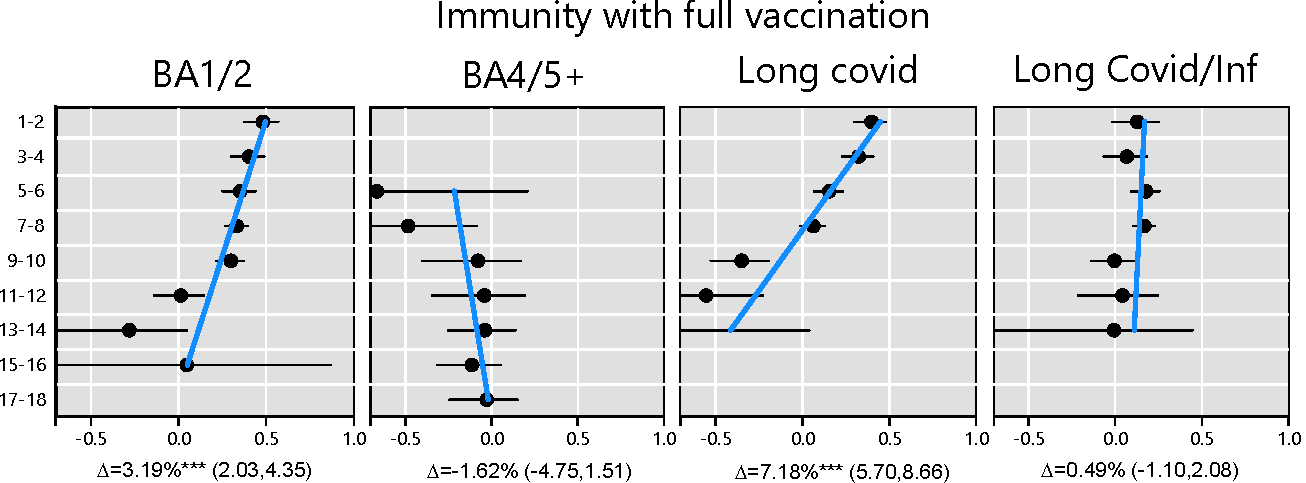
\includegraphics[width=\textwidth]{full_FINAL.pdf}
  \end{minipage}%
  \hfill
  \begin{minipage}[b]{0.48\textwidth}
    \centering
    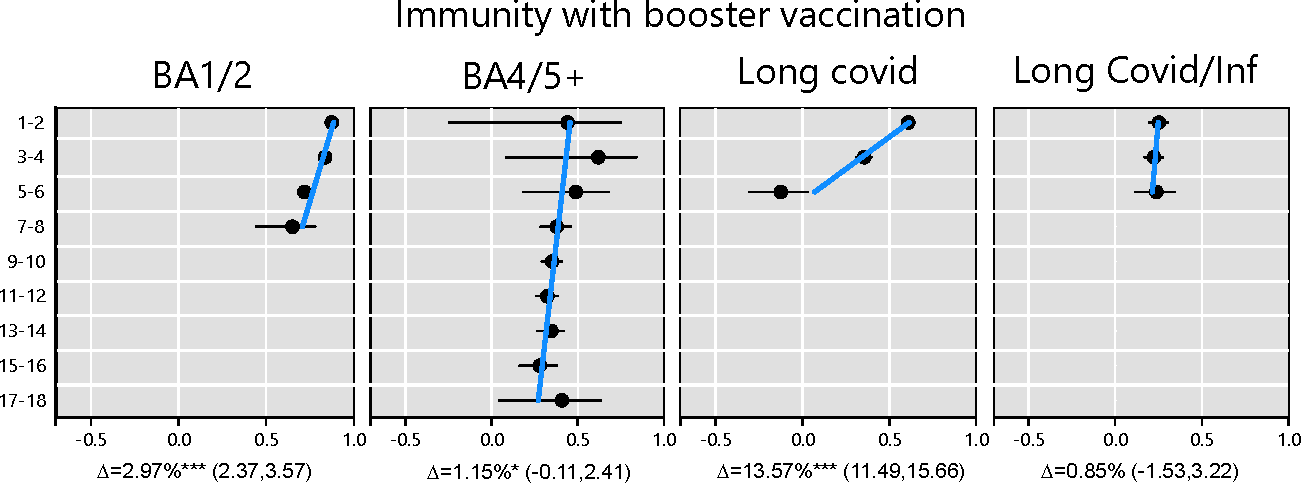
\includegraphics[width=\textwidth]{booster_FINAL.pdf}
  \end{minipage}
\vspace{3mm}\\
  \begin{minipage}[b]{0.48\textwidth}
    \centering
    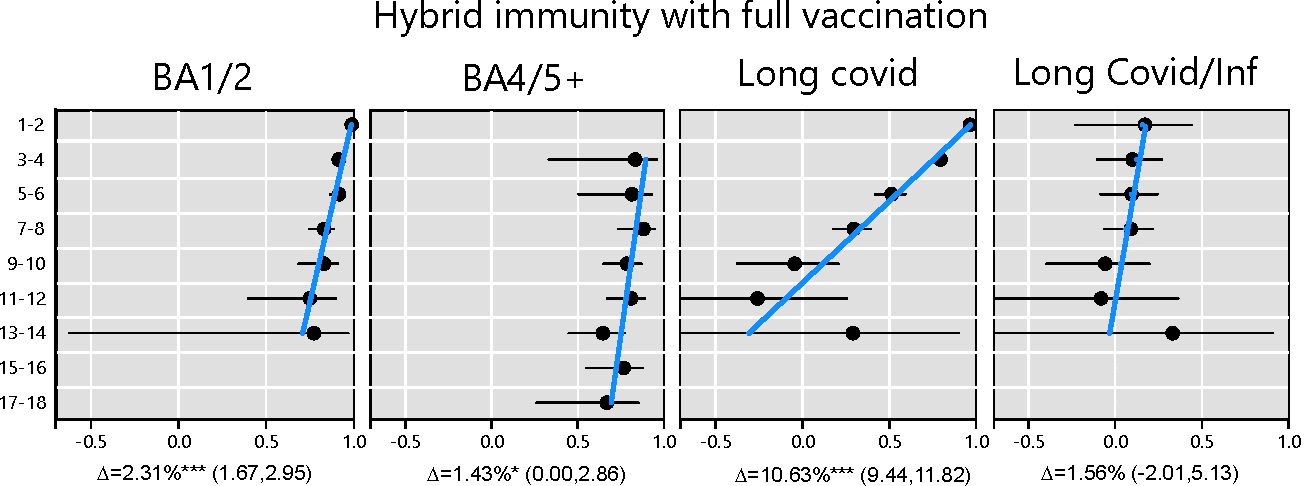
\includegraphics[width=\textwidth]{hybridfull_FINAL.pdf}
  \end{minipage}%
  \hfill
  \begin{minipage}[b]{0.48\textwidth}
    \centering
    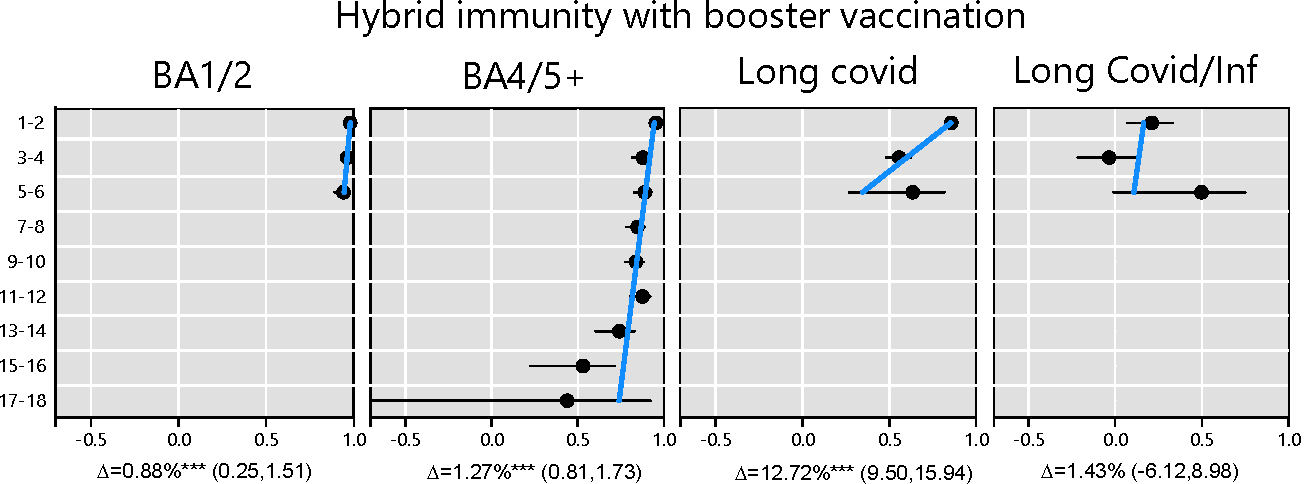
\includegraphics[width=\textwidth]{hybridbooster_FINAL.pdf}
  \end{minipage}
\vspace{3mm}\\
  \begin{minipage}[b]{0.48\textwidth}
    \centering
    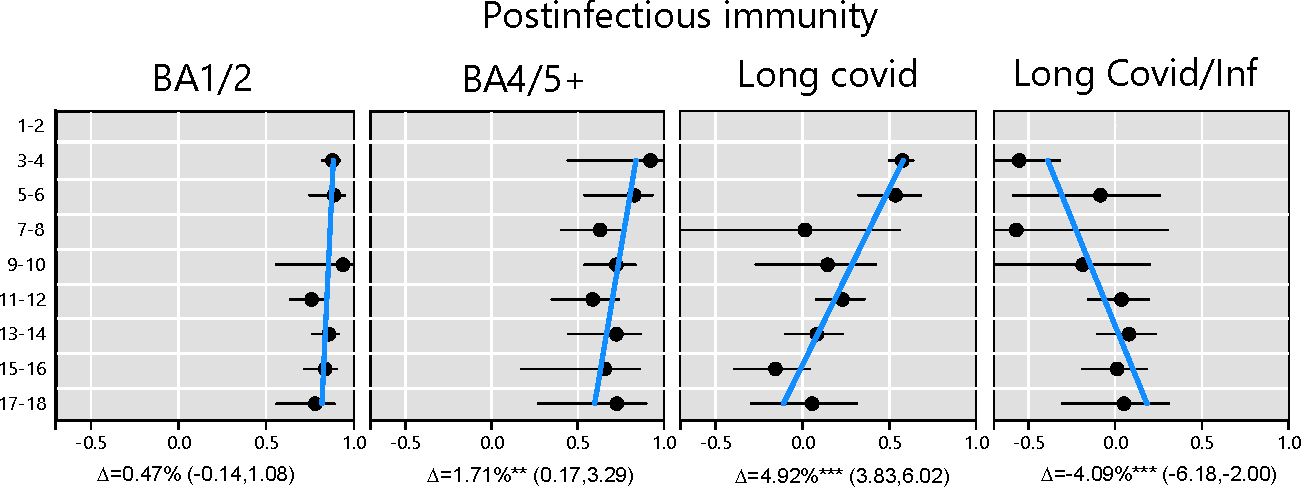
\includegraphics[width=\textwidth]{inf_FINAL.pdf}
   \end{minipage}
   \hspace{0.045\textwidth}
  \begin{minipage}[b]{0.46\textwidth}
    \centering
   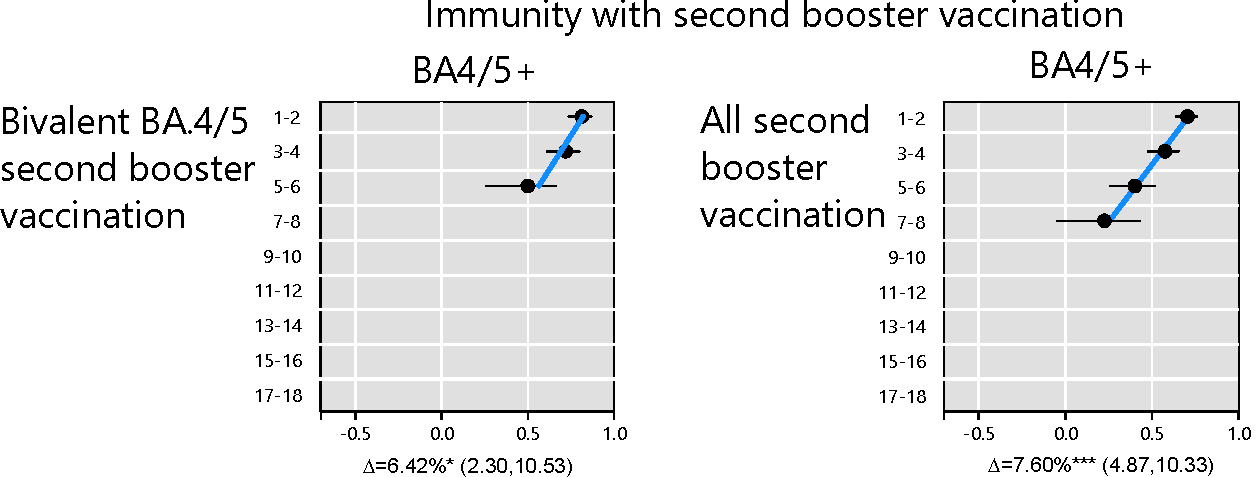
\includegraphics[width=\textwidth]{2secboosters_FINAL.pdf}
   
  \end{minipage}
\caption{TODO}
\label{trends}
\end{sidewaysfigure}

\begin{figure}
\begin{subfigure}{6cm}
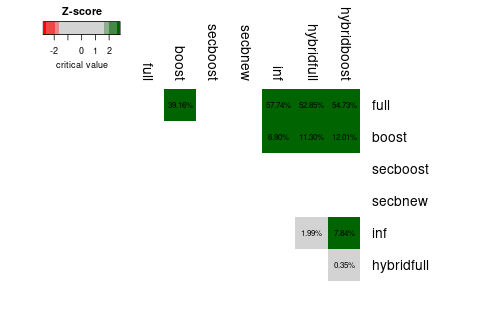
\includegraphics[width=6cm]{ProxyBA12H.png}
\caption{BA12}
\label{heatmapBA12}
\end{subfigure}
\begin{subfigure}{6cm}
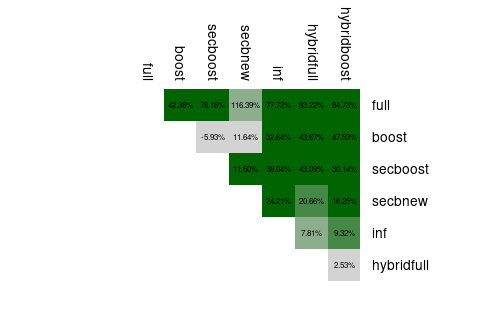
\includegraphics[width=6cm]{ProxyNewN.png}
\caption{BA45+}
\label{heatmapBA45}
\end{subfigure}\\
\begin{subfigure}{6cm}
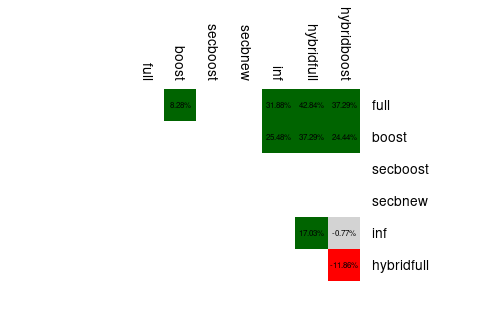
\includegraphics[width=6cm]{LCAllN.png}
\caption{LC}
\label{heatmapLC}
\end{subfigure}
\begin{subfigure}{6cm}
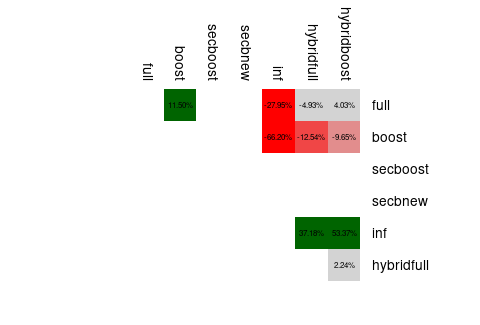
\includegraphics[width=6cm]{LCInfN.png}
\caption{LC/Inf}
\label{heatmapLCINF}
\end{subfigure}
\label{heatmaps}
\end{figure}

% Milanova tabulka
\begin{table}
\rotatebox{90}{
\begin{tabular}{ | p{1,8cm} | c  c  c  c | c  c  c  c  c | c | } 
  \hline
   & \multicolumn{4}{c|}{2021} & \multicolumn{4}{c|}{2022} & 2023 & legend \\
   \hline
   & Q1 & Q2 & Q3 & Q4 & Q1 & Q2 & Q3 & Q4 & Q1 & \\
   \hline
   &\multicolumn{9}{l|}{Infections} & \\
   \hline
By intervals of prevalence &
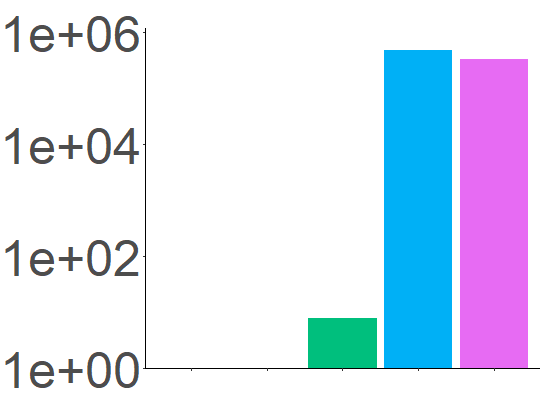
\includegraphics[height=1.1cm]{images/graph_01a_inf_01_with_scale.png}& 
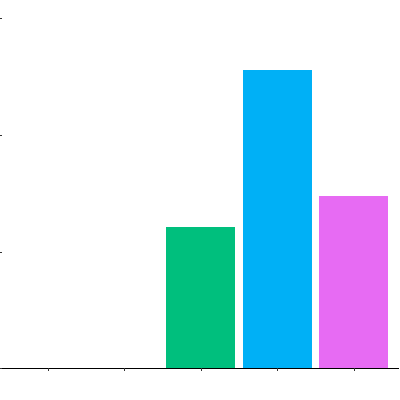
\includegraphics[height=1.1cm]{images/graph_01a_inf_02.png}&
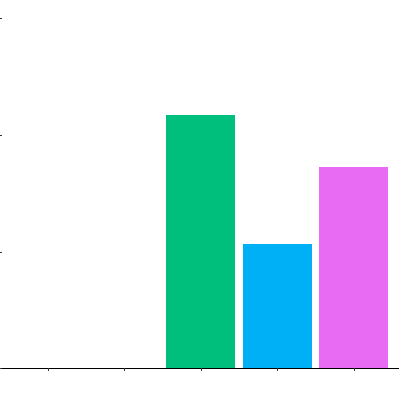
\includegraphics[height=1.1cm]{images/graph_01a_inf_03.png}&
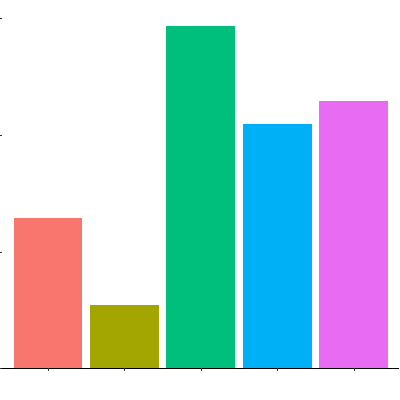
\includegraphics[height=1.1cm]{images/graph_01a_inf_04.png}&
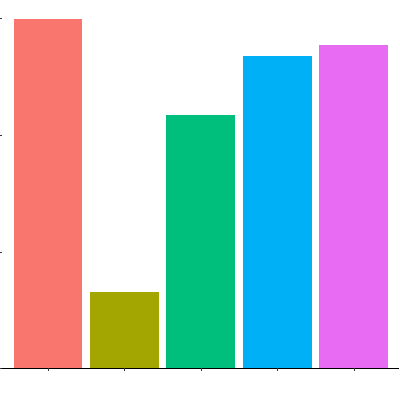
\includegraphics[height=1.1cm]{images/graph_01a_inf_05.png}&
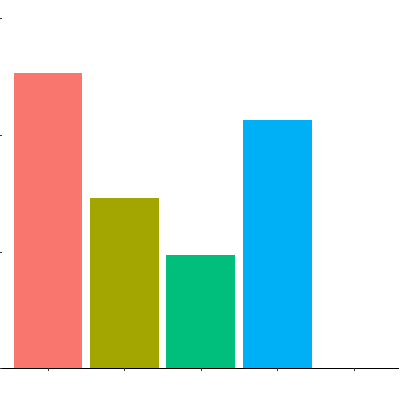
\includegraphics[height=1.1cm]{images/graph_01a_inf_06.png}&
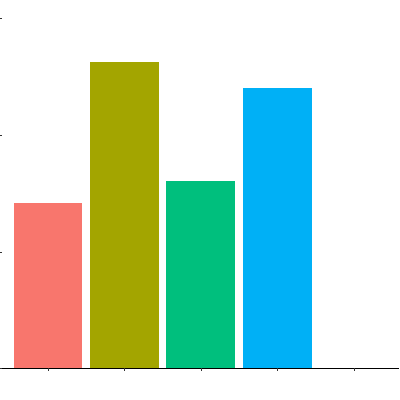
\includegraphics[height=1.1cm]{images/graph_01a_inf_07.png}&
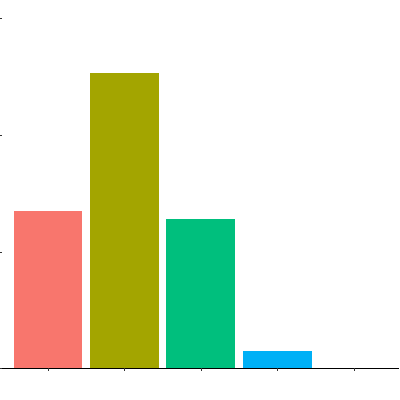
\includegraphics[height=1.1cm]{images/graph_01a_inf_08.png}&
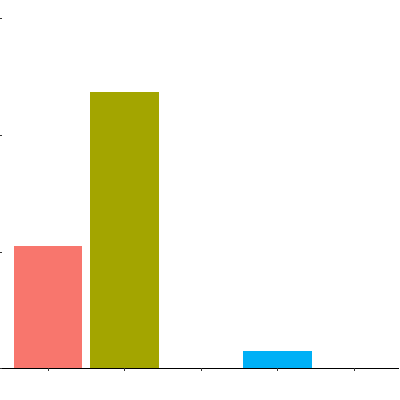
\includegraphics[height=1.1cm]{images/graph_01a_inf_09.png}&
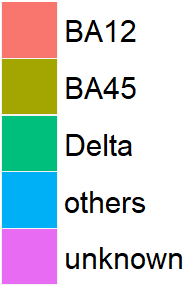
\includegraphics[height=1.1cm]{images/graph_01a_legend.png}
\\ 
   \hline 
By allele-discrimination  & 
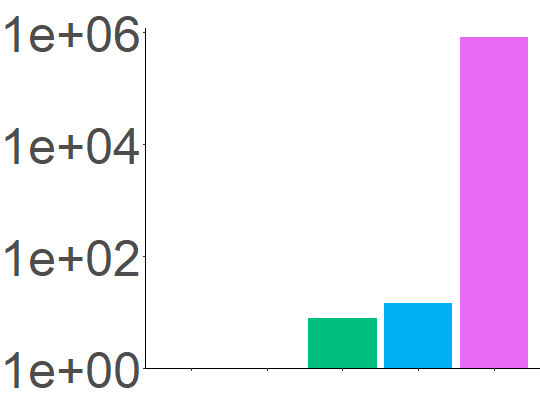
\includegraphics[height=1.1cm]{images/graph_02a_inf_01_with_scale.png} & 
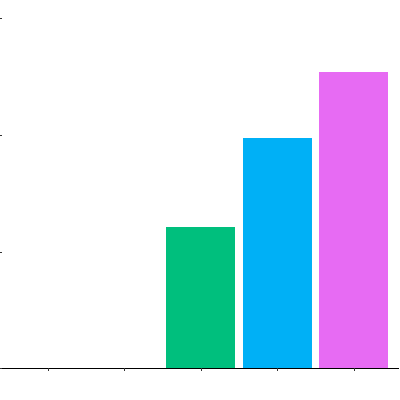
\includegraphics[height=1.1cm]{images/graph_02a_inf_02.png} &
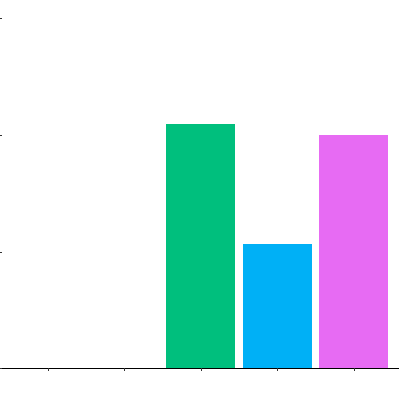
\includegraphics[height=1.1cm]{images/graph_02a_inf_03.png} &
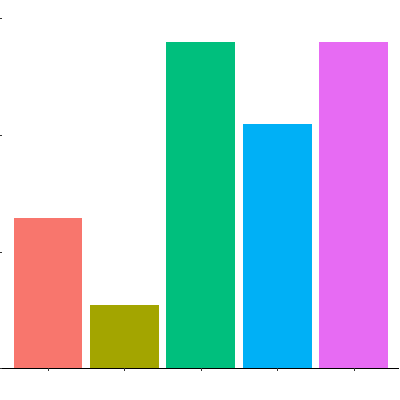
\includegraphics[height=1.1cm]{images/graph_02a_inf_04.png} &
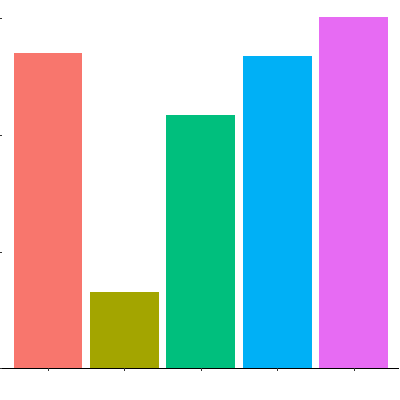
\includegraphics[height=1.1cm]{images/graph_02a_inf_05.png} &
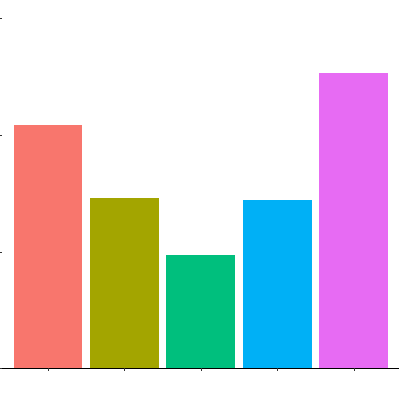
\includegraphics[height=1.1cm]{images/graph_02a_inf_06.png} &
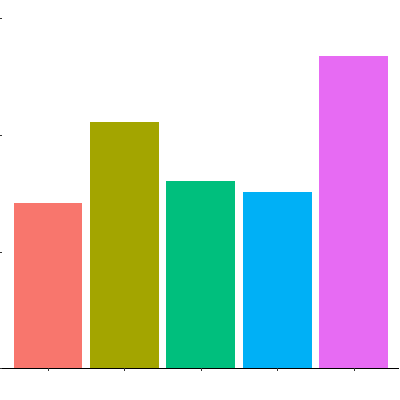
\includegraphics[height=1.1cm]{images/graph_02a_inf_07.png} &
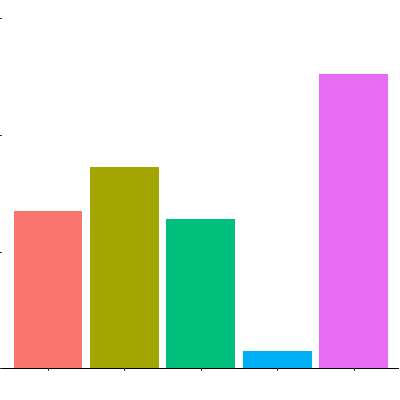
\includegraphics[height=1.1cm]{images/graph_02a_inf_08.png} &
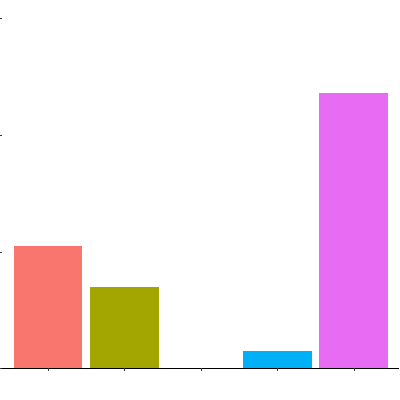
\includegraphics[height=1.1cm]{images/graph_02a_inf_09.png} &
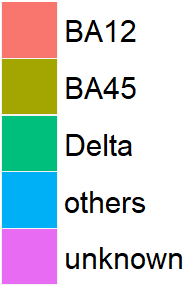
\includegraphics[height=1.1cm]{images/graph_02a_legend.png}
\\  
   \hline
\% of discriminated    & \multicolumn{9}{c|}{} &\\
   \hline
   & \multicolumn{9}{|l|}{Outcomes} &\\
   \hline
Serious courese & 
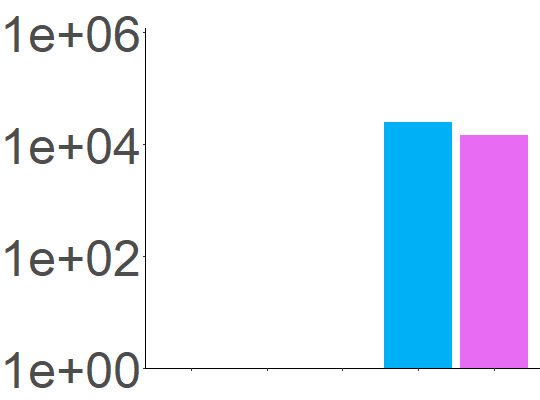
\includegraphics[height=1.1cm]{images/graph_04a_inf_01_with_scale.png} & 
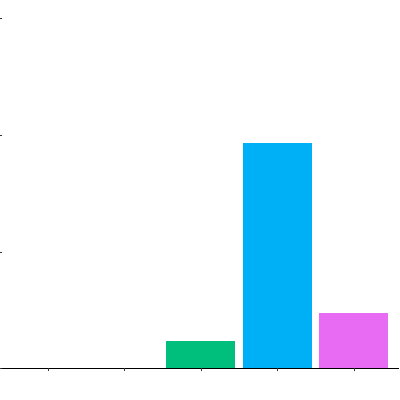
\includegraphics[height=1.1cm]{images/graph_04a_inf_02.png} &
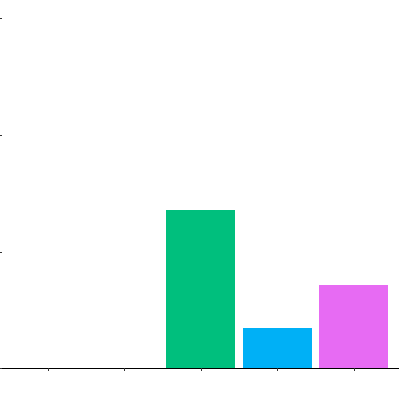
\includegraphics[height=1.1cm]{images/graph_04a_inf_03.png} &
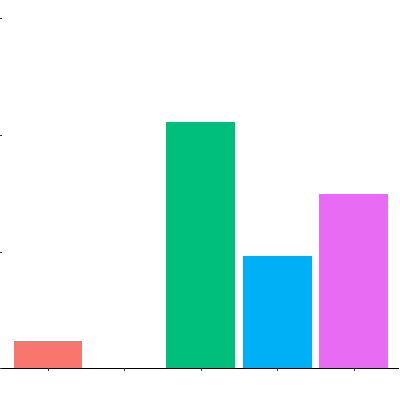
\includegraphics[height=1.1cm]{images/graph_04a_inf_04.png} &
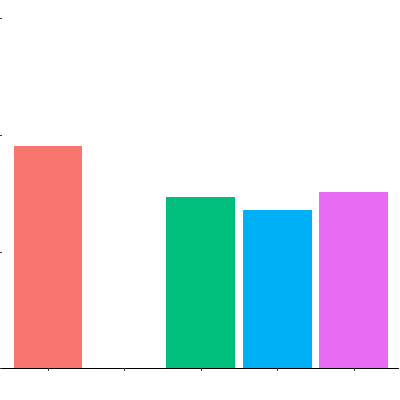
\includegraphics[height=1.1cm]{images/graph_04a_inf_05.png} &
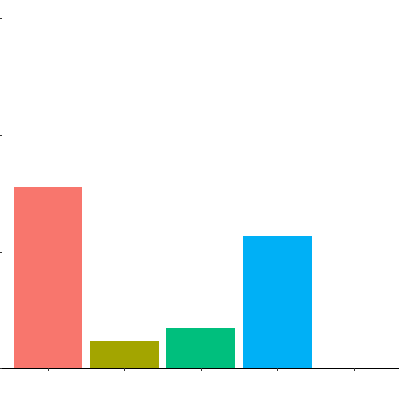
\includegraphics[height=1.1cm]{images/graph_04a_inf_06.png} &
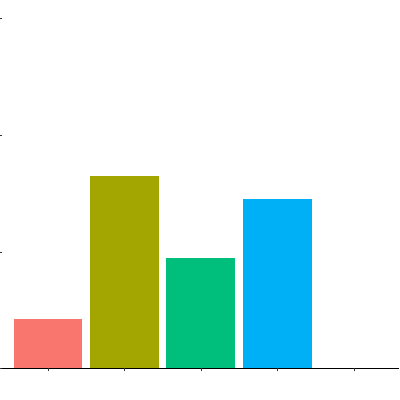
\includegraphics[height=1.1cm]{images/graph_04a_inf_07.png} &
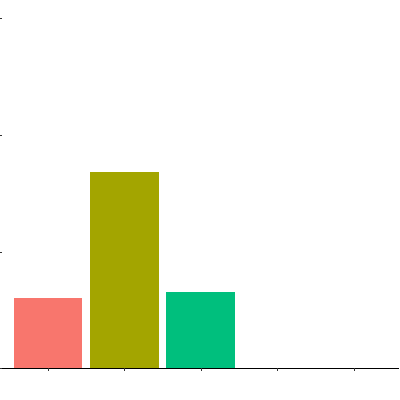
\includegraphics[height=1.1cm]{images/graph_04a_inf_08.png} &
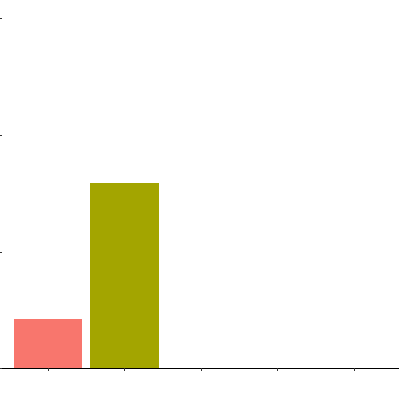
\includegraphics[height=1.1cm]{images/graph_04a_inf_09.png} &
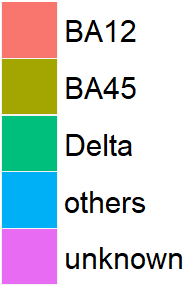
\includegraphics[height=1.1cm]{images/graph_04a_legend.png}
\\
   \hline
Long covid    & 
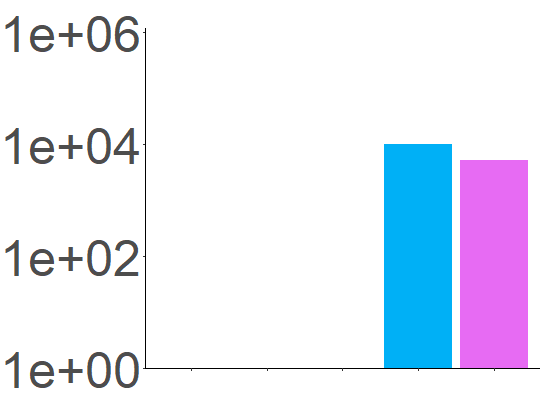
\includegraphics[height=1.1cm]{images/graph_05a_inf_01_with_scale.png} & 
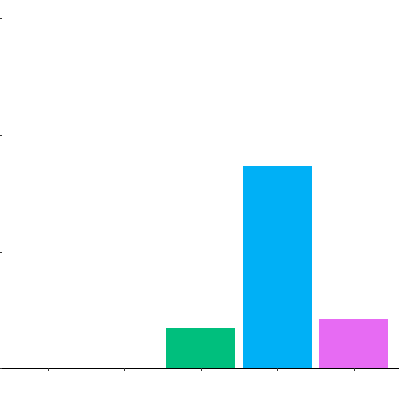
\includegraphics[height=1.1cm]{images/graph_05a_inf_02.png} &
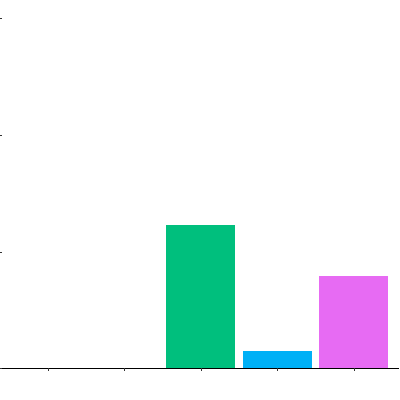
\includegraphics[height=1.1cm]{images/graph_05a_inf_03.png} &
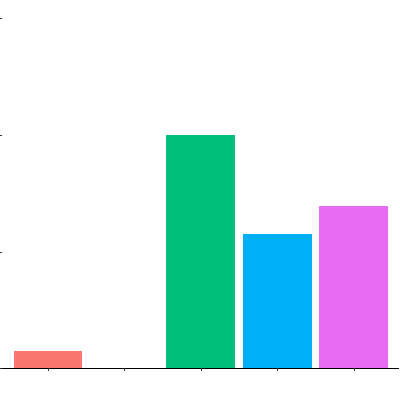
\includegraphics[height=1.1cm]{images/graph_05a_inf_04.png} &
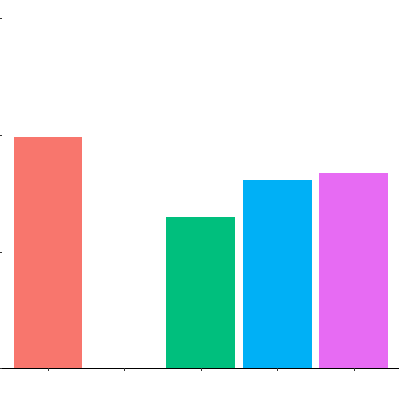
\includegraphics[height=1.1cm]{images/graph_05a_inf_05.png} &
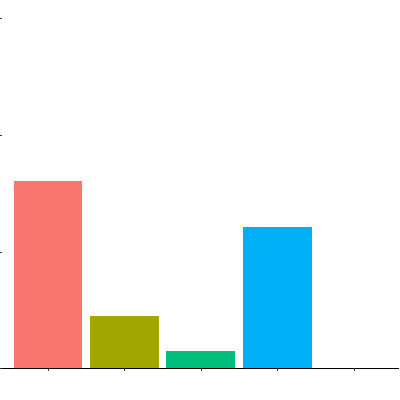
\includegraphics[height=1.1cm]{images/graph_05a_inf_06.png} &
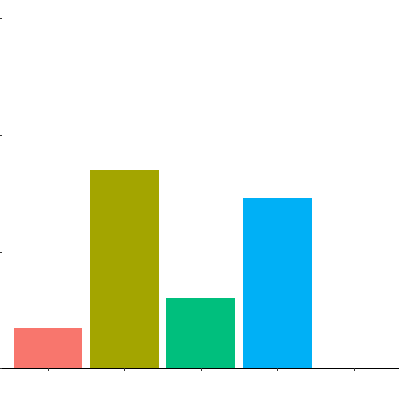
\includegraphics[height=1.1cm]{images/graph_05a_inf_07.png} &
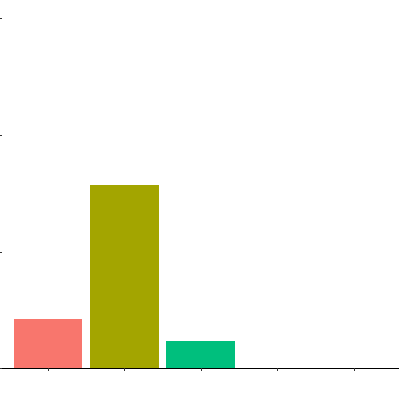
\includegraphics[height=1.1cm]{images/graph_05a_inf_08.png} &
% 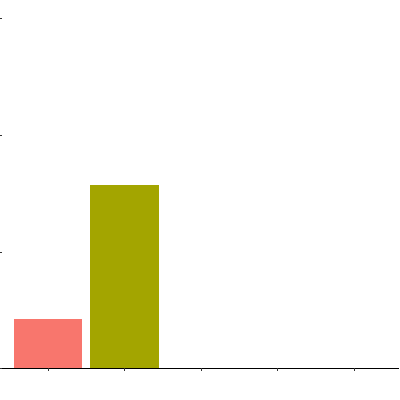
\includegraphics[height=1.1cm]{images/graph_05a_inf_09.png} &
&
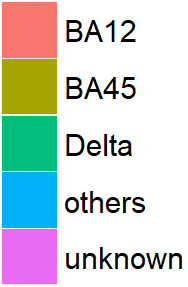
\includegraphics[height=1.1cm]{images/graph_05a_legend.png}
\\
   \hline
   & \multicolumn{9}{|l|}{Vaccination} & \\
   \hline
Full other & 
\includegraphics[height=1.1cm]{images/graph_06_inf_01_with_scale.png} & 
\includegraphics[height=1.1cm]{images/graph_06_inf_02.png} &
\includegraphics[height=1.1cm]{images/graph_06_inf_03.png} &
\includegraphics[height=1.1cm]{images/graph_06_inf_04.png} &
\includegraphics[height=1.1cm]{images/graph_06_inf_05.png} &
\includegraphics[height=1.1cm]{images/graph_06_inf_06.png} &
\includegraphics[height=1.1cm]{images/graph_06_inf_07.png} &
\includegraphics[height=1.1cm]{images/graph_06_inf_08.png} &
\includegraphics[height=1.1cm]{images/graph_06_inf_09.png} &
\includegraphics[height=1.1cm]{images/graph_06_legend.png}
\\
   \hline
Booster    & 
\includegraphics[height=1.1cm]{images/graph_07_inf_01_with_scale.png} & 
\includegraphics[height=1.1cm]{images/graph_07_inf_02.png} &
\includegraphics[height=1.1cm]{images/graph_07_inf_03.png} &
\includegraphics[height=1.1cm]{images/graph_07_inf_04.png} &
\includegraphics[height=1.1cm]{images/graph_07_inf_05.png} &
\includegraphics[height=1.1cm]{images/graph_07_inf_06.png} &
\includegraphics[height=1.1cm]{images/graph_07_inf_07.png} &
\includegraphics[height=1.1cm]{images/graph_07_inf_08.png} &
\includegraphics[height=1.1cm]{images/graph_07_inf_09.png} &
\includegraphics[height=1.1cm]{images/graph_06_legend.png}
\\
 \hline
2nd booster    & 
\includegraphics[height=1.1cm]{images/graph_08_inf_01_with_scale.png} & 
\includegraphics[height=1.1cm]{images/graph_08_inf_02.png} &
\includegraphics[height=1.1cm]{images/graph_08_inf_03.png} &
\includegraphics[height=1.1cm]{images/graph_08_inf_04.png} &
\includegraphics[height=1.1cm]{images/graph_08_inf_05.png} &
\includegraphics[height=1.1cm]{images/graph_08_inf_06.png} &
\includegraphics[height=1.1cm]{images/graph_08_inf_07.png} &
\includegraphics[height=1.1cm]{images/graph_08_inf_08.png} &
\includegraphics[height=1.1cm]{images/graph_08_inf_09.png} &
\includegraphics[height=1.1cm]{images/graph_06_legend.png}
\\
 \hline
\end{tabular}
}
\caption{Tabulka rozpracovaná další se ladí, logaritmická stupnice na ose y.}
\end{table}


\section{Discussion}


TBDMS Under-reporting

TBDTP(co tě napadá co by mohlo být napadnutelné)

TBDUZIS() 

TBDMARTIN(using intervals)

Antiviral treatment of COVID-19 disease is indicated in adult patients who are at increased risk of progression to the severe form COVID-19 disease and it became widely available during omicron dominant period (for example, Paxlovid only became available on prescription in pharmacies in the BA4/5+ period). As unvaccinated, in addition to age and comorbidities, is considered an increased risk, it may bias the results for comparing types of immunity against each other, but not the waning of various immunity types studied by us, because covariates of age and comorbidities are included in the analysis, whereas the type of prior acquired immunity is the same in a given immunity group.

\section{various}
The study was approved by the Director of the Institute of Health Information and Statistics of the Czech Republic and does not require ethical approval.

\bibliography{v3bib}

TBDMARTIN(appendix)


\end{document}

In this study, the limited number of SARS-CoV-2 sequencing data available necessitated the use of periods in which variants were highly dominant to accurately distinguish between variants during our calculations. According to data published by GISAID via CoVariants.org, the Alpha variant was dominant from February 15, 2021, to June 21, 2021, with a prevalence above 74\% (above 80\% except for one week, which may be a selection effect). The Delta variant was dominant from July 19, 2021, to December 20, 2021, with a prevalence above 97\% according to sequencing data. The Omicron BA1/2 variant was dominant from January 31, 2022, to May 23, 2022, with a prevalence over 94\% by sequencing. The Omicron BA4/5 variant was dominant from August 1, 2022, to October 24, 2022, with a prevalence above 95\% by sequencing. Currently, the Omicron variants, including XBB and BQ.1, still dominate almost 100\% of COVID-19 cases. 


\section{Introduction}\label{sec1}

The Introduction section, of referenced text \cite{bib1} expands on the background of the work (some overlap with the Abstract is acceptable). The introduction should not include subheadings.

Springer Nature does not impose a strict layout as standard however authors are advised to check the individual requirements for the journal they are planning to submit to as there may be journal-level preferences. When preparing your text please also be aware that some stylistic choices are not supported in full text XML (publication version), including coloured font. These will not be replicated in the typeset article if it is accepted. 

\section{Results}\label{sec2}

Sample body text. Sample body text. Sample body text. Sample body text. Sample body text. Sample body text. Sample body text. Sample body text.

\section{This is an example for first level head---section head}\label{sec3}

\subsection{This is an example for second level head---subsection head}\label{subsec2}

\subsubsection{This is an example for third level head---subsubsection head}\label{subsubsec2}

Sample body text. Sample body text. Sample body text. Sample body text. Sample body text. Sample body text. Sample body text. Sample body text. 

\section{Equations}\label{sec4}

Equations in \LaTeX\ can either be inline or on-a-line by itself (``display equations''). For
inline equations use the \verb+$...$+ commands. E.g.: The equation
$H\psi = E \psi$ is written via the command \verb+$H \psi = E \psi$+.

For display equations (with auto generated equation numbers)
one can use the equation or align environments:
\begin{equation}
\|\tilde{X}(k)\|^2 \leq\frac{\sum\limits_{i=1}^{p}\left\|\tilde{Y}_i(k)\right\|^2+\sum\limits_{j=1}^{q}\left\|\tilde{Z}_j(k)\right\|^2 }{p+q}.\label{eq1}
\end{equation}
where,
\begin{align}
D_\mu &=  \partial_\mu - ig \frac{\lambda^a}{2} A^a_\mu \nonumber \\
F^a_{\mu\nu} &= \partial_\mu A^a_\nu - \partial_\nu A^a_\mu + g f^{abc} A^b_\mu A^a_\nu \label{eq2}
\end{align}
Notice the use of \verb+\nonumber+ in the align environment at the end
of each line, except the last, so as not to produce equation numbers on
lines where no equation numbers are required. The \verb+\label{}+ command
should only be used at the last line of an align environment where
\verb+\nonumber+ is not used.
\begin{equation}
Y_\infty = \left( \frac{m}{\textrm{GeV}} \right)^{-3}
    \left[ 1 + \frac{3 \ln(m/\textrm{GeV})}{15}
    + \frac{\ln(c_2/5)}{15} \right]
\end{equation}
The class file also supports the use of \verb+\mathbb{}+, \verb+\mathscr{}+ and
\verb+\mathcal{}+ commands. As such \verb+\mathbb{R}+, \verb+\mathscr{R}+
and \verb+\mathcal{R}+ produces $\mathbb{R}$, $\mathscr{R}$ and $\mathcal{R}$
respectively (refer Subsubsection~\ref{subsubsec2}).

\section{Tables}\label{sec5}

Tables can be inserted via the normal table and tabular environment. To put
footnotes inside tables you should use \verb+\footnotetext[]{...}+ tag.
The footnote appears just below the table itself (refer Tables~\ref{tab1} and \ref{tab2}). 
For the corresponding footnotemark use \verb+\footnotemark[...]+

\begin{table}[h]
\begin{center}
\begin{minipage}{174pt}
\caption{Caption text}\label{tab1}%
\begin{tabular}{@{}llll@{}}
\toprule
Column 1 & Column 2  & Column 3 & Column 4\\
\midrule
row 1    & data 1   & data 2  & data 3  \\
row 2    & data 4   & data 5\footnotemark[1]  & data 6  \\
row 3    & data 7   & data 8  & data 9\footnotemark[2]  \\
\botrule
\end{tabular}
\footnotetext{Source: This is an example of table footnote. This is an example of table footnote.}
\footnotetext[1]{Example for a first table footnote. This is an example of table footnote.}
\footnotetext[2]{Example for a second table footnote. This is an example of table footnote.}
\end{minipage}
\end{center}
\end{table}

\noindent
The input format for the above table is as follows:

%%=============================================%%
%% For presentation purpose, we have included  %%
%% \bigskip command. please ignore this.       %%
%%=============================================%%
\bigskip
\begin{verbatim}
\begin{table}[<placement-specifier>]
\begin{center}
\begin{minipage}{<preferred-table-width>}
\caption{<table-caption>}\label{<table-label>}%
\begin{tabular}{@{}llll@{}}
\toprule
Column 1 & Column 2 & Column 3 & Column 4\\
\midrule
row 1 & data 1 & data 2	 & data 3 \\
row 2 & data 4 & data 5\footnotemark[1] & data 6 \\
row 3 & data 7 & data 8	 & data 9\footnotemark[2]\\
\botrule
\end{tabular}
\footnotetext{Source: This is an example of table footnote. 
This is an example of table footnote.}
\footnotetext[1]{Example for a first table footnote.
This is an example of table footnote.}
\footnotetext[2]{Example for a second table footnote. 
This is an example of table footnote.}
\end{minipage}
\end{center}
\end{table}
\end{verbatim}
\bigskip
%%=============================================%%
%% For presentation purpose, we have included  %%
%% \bigskip command. please ignore this.       %%
%%=============================================%%

\begin{table}[h]
\begin{center}
\begin{minipage}{\textwidth}
\caption{Example of a lengthy table which is set to full textwidth}\label{tab2}
\begin{tabular*}{\textwidth}{@{\extracolsep{\fill}}lcccccc@{\extracolsep{\fill}}}
\toprule%
& \multicolumn{3}{@{}c@{}}{Element 1\footnotemark[1]} & \multicolumn{3}{@{}c@{}}{Element 2\footnotemark[2]} \\\cmidrule{2-4}\cmidrule{5-7}%
Project & Energy & $\sigma_{calc}$ & $\sigma_{expt}$ & Energy & $\sigma_{calc}$ & $\sigma_{expt}$ \\
\midrule
Element 3  & 990 A & 1168 & $1547\pm12$ & 780 A & 1166 & $1239\pm100$\\
Element 4  & 500 A & 961  & $922\pm10$  & 900 A & 1268 & $1092\pm40$\\
\botrule
\end{tabular*}
\footnotetext{Note: This is an example of table footnote. This is an example of table footnote this is an example of table footnote this is an example of~table footnote this is an example of table footnote.}
\footnotetext[1]{Example for a first table footnote.}
\footnotetext[2]{Example for a second table footnote.}
\end{minipage}
\end{center}
\end{table}

In case of double column layout, tables which do not fit in single column width should be set to full text width. For this, you need to use \verb+\begin{table*}+ \verb+...+ \verb+\end{table*}+ instead of \verb+\begin{table}+ \verb+...+ \verb+\end{table}+ environment. Lengthy tables which do not fit in textwidth should be set as rotated table. For this, you need to use \verb+\begin{sidewaystable}+ \verb+...+ \verb+\end{sidewaystable}+ instead of \verb+\begin{table*}+ \verb+...+ \verb+\end{table*}+ environment. This environment puts tables rotated to single column width. For tables rotated to double column width, use \verb+\begin{sidewaystable*}+ \verb+...+ \verb+\end{sidewaystable*}+.

\begin{sidewaystable}
\sidewaystablefn%
\begin{center}
\begin{minipage}{\textheight}
\caption{Tables which are too long to fit, should be written using the ``sidewaystable'' environment as shown here}\label{tab3}
\begin{tabular*}{\textheight}{@{\extracolsep{\fill}}lcccccc@{\extracolsep{\fill}}}
\toprule%
& \multicolumn{3}{@{}c@{}}{Element 1\footnotemark[1]}& \multicolumn{3}{@{}c@{}}{Element\footnotemark[2]} \\\cmidrule{2-4}\cmidrule{5-7}%
Projectile & Energy	& $\sigma_{calc}$ & $\sigma_{expt}$ & Energy & $\sigma_{calc}$ & $\sigma_{expt}$ \\
\midrule
Element 3 & 990 A & 1168 & $1547\pm12$ & 780 A & 1166 & $1239\pm100$ \\
Element 4 & 500 A & 961  & $922\pm10$  & 900 A & 1268 & $1092\pm40$ \\
Element 5 & 990 A & 1168 & $1547\pm12$ & 780 A & 1166 & $1239\pm100$ \\
Element 6 & 500 A & 961  & $922\pm10$  & 900 A & 1268 & $1092\pm40$ \\
\botrule
\end{tabular*}
\footnotetext{Note: This is an example of table footnote this is an example of table footnote this is an example of table footnote this is an example of~table footnote this is an example of table footnote.}
\footnotetext[1]{This is an example of table footnote.}
\end{minipage}
\end{center}
\end{sidewaystable}

\section{Figures}\label{sec6}

As per the \LaTeX\ standards you need to use eps images for \LaTeX\ compilation and \verb+pdf/jpg/png+ images for \verb+PDFLaTeX+ compilation. This is one of the major difference between \LaTeX\ and \verb+PDFLaTeX+. Each image should be from a single input .eps/vector image file. Avoid using subfigures. The command for inserting images for \LaTeX\ and \verb+PDFLaTeX+ can be generalized. The package used to insert images in \verb+LaTeX/PDFLaTeX+ is the graphicx package. Figures can be inserted via the normal figure environment as shown in the below example:

%%=============================================%%
%% For presentation purpose, we have included  %%
%% \bigskip command. please ignore this.       %%
%%=============================================%%
\bigskip
\begin{verbatim}
\begin{figure}[<placement-specifier>]
\centering
\includegraphics{<eps-file>}
\caption{<figure-caption>}\label{<figure-label>}
\end{figure}
\end{verbatim}
\bigskip
%%=============================================%%
%% For presentation purpose, we have included  %%
%% \bigskip command. please ignore this.       %%
%%=============================================%%

\begin{figure}[h]%
\centering
%\includegraphics[width=0.9\textwidth]{fig.eps}
\caption{This is a widefig. This is an example of long caption this is an example of long caption  this is an example of long caption this is an example of long caption}\label{fig1}
\end{figure}

In case of double column layout, the above format puts figure captions/images to single column width. To get spanned images, we need to provide \verb+\begin{figure*}+ \verb+...+ \verb+\end{figure*}+.

For sample purpose, we have included the width of images in the optional argument of \verb+\includegraphics+ tag. Please ignore this. 

\section{Algorithms, Program codes and Listings}\label{sec7}

Packages \verb+algorithm+, \verb+algorithmicx+ and \verb+algpseudocode+ are used for setting algorithms in \LaTeX\ using the format:

%%=============================================%%
%% For presentation purpose, we have included  %%
%% \bigskip command. please ignore this.       %%
%%=============================================%%
\bigskip
\begin{verbatim}
\begin{algorithm}
\caption{<alg-caption>}\label{<alg-label>}
\begin{algorithmic}[1]
. . .
\end{algorithmic}
\end{algorithm}
\end{verbatim}
\bigskip
%%=============================================%%
%% For presentation purpose, we have included  %%
%% \bigskip command. please ignore this.       %%
%%=============================================%%

You may refer above listed package documentations for more details before setting \verb+algorithm+ environment. For program codes, the ``program'' package is required and the command to be used is \verb+\begin{program}+ \verb+...+ \verb+\end{program}+. A fast exponentiation procedure:

\begin{program}
\BEGIN \\ %
  \FOR i:=1 \TO 10 \STEP 1 \DO
     |expt|(2,i); \\ |newline|() \OD %
\rcomment{Comments will be set flush to the right margin}
\WHERE
\PROC |expt|(x,n) \BODY
          z:=1;
          \DO \IF n=0 \THEN \EXIT \FI;
             \DO \IF |odd|(n) \THEN \EXIT \FI;
\COMMENT{This is a comment statement};
                n:=n/2; x:=x*x \OD;
             \{ n>0 \};
             n:=n-1; z:=z*x \OD;
          |print|(z) \ENDPROC
\END
\end{program}


\begin{algorithm}
\caption{Calculate $y = x^n$}\label{algo1}
\begin{algorithmic}[1]
\Require $n \geq 0 \vee x \neq 0$
\Ensure $y = x^n$ 
\State $y \Leftarrow 1$
\If{$n < 0$}\label{algln2}
        \State $X \Leftarrow 1 / x$
        \State $N \Leftarrow -n$
\Else
        \State $X \Leftarrow x$
        \State $N \Leftarrow n$
\EndIf
\While{$N \neq 0$}
        \If{$N$ is even}
            \State $X \Leftarrow X \times X$
            \State $N \Leftarrow N / 2$
        \Else[$N$ is odd]
            \State $y \Leftarrow y \times X$
            \State $N \Leftarrow N - 1$
        \EndIf
\EndWhile
\end{algorithmic}
\end{algorithm}
\bigskip
%%=============================================%%
%% For presentation purpose, we have included  %%
%% \bigskip command. please ignore this.       %%
%%=============================================%%

Similarly, for \verb+listings+, use the \verb+listings+ package. \verb+\begin{lstlisting}+ \verb+...+ \verb+\end{lstlisting}+ is used to set environments similar to \verb+verbatim+ environment. Refer to the \verb+lstlisting+ package documentation for more details.

%%=============================================%%
%% For presentation purpose, we have included  %%
%% \bigskip command. please ignore this.       %%
%%=============================================%%
\bigskip
\begin{minipage}{\hsize}%
\lstset{frame=single,framexleftmargin=-1pt,framexrightmargin=-17pt,framesep=12pt,linewidth=0.98\textwidth,language=pascal}% Set your language (you can change the language for each code-block optionally)
%%% Start your code-block
\begin{lstlisting}
for i:=maxint to 0 do
begin
{ do nothing }
end;
Write('Case insensitive ');
Write('Pascal keywords.');
\end{lstlisting}
\end{minipage}

\section{Cross referencing}\label{sec8}

Environments such as figure, table, equation and align can have a label
declared via the \verb+\label{#label}+ command. For figures and table
environments use the \verb+\label{}+ command inside or just
below the \verb+\caption{}+ command. You can then use the
\verb+\ref{#label}+ command to cross-reference them. As an example, consider
the label declared for Figure~\ref{fig1} which is
\verb+\label{fig1}+. To cross-reference it, use the command 
\verb+Figure \ref{fig1}+, for which it comes up as
``Figure~\ref{fig1}''. 

To reference line numbers in an algorithm, consider the label declared for the line number 2 of Algorithm~\ref{algo1} is \verb+\label{algln2}+. To cross-reference it, use the command \verb+\ref{algln2}+ for which it comes up as line~\ref{algln2} of Algorithm~\ref{algo1}.

\subsection{Details on reference citations}\label{subsec7}

Standard \LaTeX\ permits only numerical citations. To support both numerical and author-year citations this template uses \verb+natbib+ \LaTeX\ package. For style guidance please refer to the template user manual.

Here is an example for \verb+\cite{...}+: \cite{bib1}. Another example for \verb+\citep{...}+: \citep{bib2}. For author-year citation mode, \verb+\cite{...}+ prints Jones et al. (1990) and \verb+\citep{...}+ prints (Jones et al., 1990).

All cited bib entries are printed at the end of this article: \cite{bib3}, \cite{bib4}, \cite{bib5}, \cite{bib6}, \cite{bib7}, \cite{bib8}, \cite{bib9}, \cite{bib10}, \cite{bib11} and \cite{bib12}.

\section{Examples for theorem like environments}\label{sec10}

For theorem like environments, we require \verb+amsthm+ package. There are three types of predefined theorem styles exists---\verb+thmstyleone+, \verb+thmstyletwo+ and \verb+thmstylethree+ 

%%=============================================%%
%% For presentation purpose, we have included  %%
%% \bigskip command. please ignore this.       %%
%%=============================================%%
\bigskip
\begin{tabular}{|l|p{19pc}|}
\hline
\verb+thmstyleone+ & Numbered, theorem head in bold font and theorem text in italic style \\\hline
\verb+thmstyletwo+ & Numbered, theorem head in roman font and theorem text in italic style \\\hline
\verb+thmstylethree+ & Numbered, theorem head in bold font and theorem text in roman style \\\hline
\end{tabular}
\bigskip
%%=============================================%%
%% For presentation purpose, we have included  %%
%% \bigskip command. please ignore this.       %%
%%=============================================%%

For mathematics journals, theorem styles can be included as shown in the following examples:

\begin{theorem}[Theorem subhead]\label{thm1}
Example theorem text. Example theorem text. Example theorem text. Example theorem text. Example theorem text. 
Example theorem text. Example theorem text. Example theorem text. Example theorem text. Example theorem text. 
Example theorem text. 
\end{theorem}

Sample body text. Sample body text. Sample body text. Sample body text. Sample body text. Sample body text. Sample body text. Sample body text.

\begin{proposition}
Example proposition text. Example proposition text. Example proposition text. Example proposition text. Example proposition text. 
Example proposition text. Example proposition text. Example proposition text. Example proposition text. Example proposition text. 
\end{proposition}

Sample body text. Sample body text. Sample body text. Sample body text. Sample body text. Sample body text. Sample body text. Sample body text.

\begin{example}
Phasellus adipiscing semper elit. Proin fermentum massa
ac quam. Sed diam turpis, molestie vitae, placerat a, molestie nec, leo. Maecenas lacinia. Nam ipsum ligula, eleifend
at, accumsan nec, suscipit a, ipsum. Morbi blandit ligula feugiat magna. Nunc eleifend consequat lorem. 
\end{example}

Sample body text. Sample body text. Sample body text. Sample body text. Sample body text. Sample body text. Sample body text. Sample body text.

\begin{remark}
Phasellus adipiscing semper elit. Proin fermentum massa
ac quam. Sed diam turpis, molestie vitae, placerat a, molestie nec, leo. Maecenas lacinia. Nam ipsum ligula, eleifend
at, accumsan nec, suscipit a, ipsum. Morbi blandit ligula feugiat magna. Nunc eleifend consequat lorem. 
\end{remark}

Sample body text. Sample body text. Sample body text. Sample body text. Sample body text. Sample body text. Sample body text. Sample body text.

\begin{definition}[Definition sub head]
Example definition text. Example definition text. Example definition text. Example definition text. Example definition text. Example definition text. Example definition text. Example definition text. 
\end{definition}

Additionally a predefined ``proof'' environment is available: \verb+\begin{proof}+ \verb+...+ \verb+\end{proof}+. This prints a ``Proof'' head in italic font style and the ``body text'' in roman font style with an open square at the end of each proof environment. 

\begin{proof}
Example for proof text. Example for proof text. Example for proof text. Example for proof text. Example for proof text. Example for proof text. Example for proof text. Example for proof text. Example for proof text. Example for proof text. 
\end{proof}

Sample body text. Sample body text. Sample body text. Sample body text. Sample body text. Sample body text. Sample body text. Sample body text.

\begin{proof}[Proof of Theorem~{\upshape\ref{thm1}}]
Example for proof text. Example for proof text. Example for proof text. Example for proof text. Example for proof text. Example for proof text. Example for proof text. Example for proof text. Example for proof text. Example for proof text. 
\end{proof}

\noindent
For a quote environment, use \verb+\begin{quote}...\end{quote}+
\begin{quote}
Quoted text example. Aliquam porttitor quam a lacus. Praesent vel arcu ut tortor cursus volutpat. In vitae pede quis diam bibendum placerat. Fusce elementum
convallis neque. Sed dolor orci, scelerisque ac, dapibus nec, ultricies ut, mi. Duis nec dui quis leo sagittis commodo.
\end{quote}

Sample body text. Sample body text. Sample body text. Sample body text. Sample body text (refer Figure~\ref{fig1}). Sample body text. Sample body text. Sample body text (refer Table~\ref{tab3}). 

\section{Methods}\label{sec11}

Topical subheadings are allowed. Authors must ensure that their Methods section includes adequate experimental and characterization data necessary for others in the field to reproduce their work. Authors are encouraged to include RIIDs where appropriate. 

\textbf{Ethical approval declarations} (only required where applicable) Any article reporting experiment/s carried out on (i)~live vertebrate (or higher invertebrates), (ii)~humans or (iii)~human samples must include an unambiguous statement within the methods section that meets the following requirements: 

\begin{enumerate}[1.]
\item Approval: a statement which confirms that all experimental protocols were approved by a named institutional and/or licensing committee. Please identify the approving body in the methods section

\item Accordance: a statement explicitly saying that the methods were carried out in accordance with the relevant guidelines and regulations

\item Informed consent (for experiments involving humans or human tissue samples): include a statement confirming that informed consent was obtained from all participants and/or their legal guardian/s
\end{enumerate}

If your manuscript includes potentially identifying patient/participant information, or if it describes human transplantation research, or if it reports results of a clinical trial then  additional information will be required. Please visit (\url{https://www.nature.com/nature-research/editorial-policies}) for Nature Portfolio journals, (\url{https://www.springer.com/gp/authors-editors/journal-author/journal-author-helpdesk/publishing-ethics/14214}) for Springer Nature journals, or (\url{https://www.biomedcentral.com/getpublished/editorial-policies\#ethics+and+consent}) for BMC.

\section{Discussion}\label{sec12}

Discussions should be brief and focused. In some disciplines use of Discussion or `Conclusion' is interchangeable. It is not mandatory to use both. Some journals prefer a section `Results and Discussion' followed by a section `Conclusion'. Please refer to Journal-level guidance for any specific requirements. 

\section{Conclusion}\label{sec13}

Conclusions may be used to restate your hypothesis or research question, restate your major findings, explain the relevance and the added value of your work, highlight any limitations of your study, describe future directions for research and recommendations. 

In some disciplines use of Discussion or 'Conclusion' is interchangeable. It is not mandatory to use both. Please refer to Journal-level guidance for any specific requirements. 

\backmatter

\bmhead{Supplementary information}

If your article has accompanying supplementary file/s please state so here. 

Authors reporting data from electrophoretic gels and blots should supply the full unprocessed scans for key as part of their Supplementary information. This may be requested by the editorial team/s if it is missing.

Please refer to Journal-level guidance for any specific requirements.

\bmhead{Acknowledgments}

Acknowledgments are not compulsory. Where included they should be brief. Grant or contribution numbers may be acknowledged.

Please refer to Journal-level guidance for any specific requirements.

\section*{Declarations}

Some journals require declarations to be submitted in a standardised format. Please check the Instructions for Authors of the journal to which you are submitting to see if you need to complete this section. If yes, your manuscript must contain the following sections under the heading `Declarations':

\begin{itemize}
\item Funding
\item Conflict of interest/Competing interests (check journal-specific guidelines for which heading to use)
\item Ethics approval 
\item Consent to participate
\item Consent for publication
\item Availability of data and materials
\item Code availability 
\item Authors' contributions
\end{itemize}

\noindent
If any of the sections are not relevant to your manuscript, please include the heading and write `Not applicable' for that section. 

%%===================================================%%
%% For presentation purpose, we have included        %%
%% \bigskip command. please ignore this.             %%
%%===================================================%%
\bigskip
\begin{flushleft}%
Editorial Policies for:

\bigskip\noindent
Springer journals and proceedings: \url{https://www.springer.com/gp/editorial-policies}

\bigskip\noindent
Nature Portfolio journals: \url{https://www.nature.com/nature-research/editorial-policies}

\bigskip\noindent
\textit{Scientific Reports}: \url{https://www.nature.com/srep/journal-policies/editorial-policies}

\bigskip\noindent
BMC journals: \url{https://www.biomedcentral.com/getpublished/editorial-policies}
\end{flushleft}

\begin{appendices}

\section{Section title of first appendix}\label{secA1}

An appendix contains supplementary information that is not an essential part of the text itself but which may be helpful in providing a more comprehensive understanding of the research problem or it is information that is too cumbersome to be included in the body of the paper.

%%=============================================%%
%% For submissions to Nature Portfolio Journals %%
%% please use the heading ``Extended Data''.   %%
%%=============================================%%

%%=============================================================%%
%% Sample for another appendix section			       %%
%%=============================================================%%

%% \section{Example of another appendix section}\label{secA2}%
%% Appendices may be used for helpful, supporting or essential material that would otherwise 
%% clutter, break up or be distracting to the text. Appendices can consist of sections, figures, 
%% tables and equations etc.

\end{appendices}

%%===========================================================================================%%
%% If you are submitting to one of the Nature Portfolio journals, using the eJP submission   %%
%% system, please include the references within the manuscript file itself. You may do this  %%
%% by copying the reference list from your .bbl file, paste it into the main manuscript .tex %%
%% file, and delete the associated \verb+\bibliography+ commands.                            %%
%%===========================================================================================%%

\bibliography{v3bib}% common bib file
%% if required, the content of .bbl file can be included here once bbl is generated
%%\input sn-article.bbl

%% Default %%
%%\input sn-sample-bib.tex%

\end{document}
